\chapter{Hierarchical models, part 1}

\section{Exercise 8.1, Hoff}

\subsection{Data}
\begin{itemize}
 \item Consider the hierarchical model where
       \begin{align*}
        \theta_1, \ldots, \theta_m   | \mu, \tau^2        & \sim \iid \Normal(\mu,
        \tau^2)
        \\
        y_{1, j}, \ldots, y_{n_j, j} | \theta_j, \sigma^2 & \sim \iid \Normal(\theta_j,
        \sigma^2)
       \end{align*}
\end{itemize}

\subsection{Questions}
\begin{enumerate}[label=\alph*)]
 \item Which do you think is bigger, $ \Var[y_{i, j} | \theta_i, \sigma^2] $ or $
        \Var[y_{i, j} | \mu, \tau^2] $?
 \item Do you think $ \Cov[y_{i_1, j}, y_{i_2, j} | \theta_j, \sigma^2] $ is negative,
       positive or zero?
       Answer the same for $ \Cov[y_{i_1, j}, y_{i_2, j} | \mu, \tau^2] $.
 \item Compute the quantities and compare with the intuitive results.
 \item Assuming that we had a prior $ p(\mu) $ for $\mu$. Using the Bayes' rule, show
       that
       \[ p(\mu | \theta_1, \ldots, \theta_m, \tau^2, \sigma^2, \vect y_1, \ldots, \vect
        y_m) =
        p(\mu | \theta_1, \ldots, \theta_m, \tau^2) \]
       Interpret in words what this means.
\end{enumerate}

\subsection{Solutions}
\begin{enumerate}[label=\alph*)]
 \item $ \Var[y_{i, j} | \mu, \tau^2] $ will be intuitively the higher one, because we
       are \textit{constraining}
       fewer variables.
 \item The two variables $ y_{i_1, j} $ and $ y_{i_2, j} $ will be independent given $
        \theta_j $, for definition.
       Yet, if I condition only on $ \mu $ and $ \tau^2 $, the two variables will have a
       positive covariance; in fact
       if I observe a high value of $ y_{i_1, j} $ I expect to see a similar value for $
        y_{i_2, j} $ and vice versa.
 \item \begin{align*}
        \intertext{\raggedleft By definition, we know that $ y_{i, j} | \theta_j,
          \sigma^2
          \sim \Normal(\theta_j, \sigma^2) $}
        \Var[y_{i, j} | \theta_j, \sigma^2]
         & = \sigma^2
        \\
        \intertext{\raggedleft We can apply the property of variance of independent
         variables,
         \\
         because $ y_{i, j} | \theta_j, \sigma^2 $ are i.i.d.}
        \Var[\bar y_j | \theta_j, \sigma^2]
         & = \Var\left[ \frac{1}{n} \sum_{i = 1}^{n} y_{i, j} | \theta_j, \sigma^2
         \right]
        \\
         & = \frac{1}{n} \sum_{i = 1}^{n} \Var[y_{i, j} | \theta_j, \sigma^2] =
        \frac{\sigma^2}{n_j}
        \\
        \intertext{\raggedleft Again using the property that $ y_{i, j} $ are i.i.d.,
         given
         $ \theta_j $ and $ \sigma^2 $}
        \Cov[y_{i_1, j}, y_{i_2, j} | \theta_j, \sigma^2]
         & = 0
        \\
        \intertext{\centering The first intuition of point b) was correct, and justified
         by theory.}
       \end{align*}

       \setlength{\fboxsep}{10pt} % increase the spacing of fbox
       \fbox{\parbox{\textwidth}{ % put everything inside a frame
         \textbf{Note} \quad This quantities concern variables conditioned to a generic
         group \textit{j},
         and it is straightforward to obtain them even in a frequentist point of view.
         The next variances require to consider these theorems of probability theory:
         \begin{enumerate}
          \item \textbf{Law of total variance}: \\
                Given two random variables $ X $ and $ Y $ with $ \Var[X] < \infty $,
                then:
                \begin{equation}\label{week7:eq_totalvariance}
                 \Var[X] = \E[\Var[X | Y]] + \Var[\E[X | Y]]
                \end{equation}
          \item \textbf{Law of total covariance}: \\
                Given three random variables $ X $, $ Y $ and $ Z $ with $ \Cov[X, Y] <
                 \infty $, then:
                \begin{equation}\label{week7:eq_totalcovariance}
                 \Cov[X, Y | Z] = \E[\Cov[X, Y | Z]] + \Cov[\E[X | Z] \cdot \E[Y | Z]]
                \end{equation}
         \end{enumerate}
        }}

       \begin{align*}
        \intertext{\raggedleft Thus, we can apply here \ref{week7:eq_totalvariance} with
         $ X = y_{i, j} $ and $ Y = \theta_j $}
        \Var[y_{i, j} | \mu, \tau^2]
         & = \E[\Var[y_{i, j} | \theta_j, \mu, \tau^2]] + \Var[\E[y_{i, j} | \theta_j,
          \mu,
          \tau^2]]
        \\
         & = \E[\Var[y_{i, j} | \theta_j, \sigma^2, \mu, \tau^2]] +
        \Var[\E[y_{i, j} | \theta_j, \sigma^2, \mu, \tau^2]]
        \\
         & = \E[\sigma^2] + \Var[\theta_j | \mu, \tau^2]
        \\
         & = \sigma^2 + \tau^2 > \sigma^2
        \\
        \intertext{\centering The intuition at point a) is confirmed.}
        \intertext{\raggedleft We apply again \ref{week7:eq_totalvariance}, with $ X =
          \bar y_j $ and $ Y = \theta_j $}
        \Var[\bar y_j | \mu, \tau^2]
         & = \E[\Var[\bar y_j | \theta_j, \mu, \tau^2]] + \Var[\E[\bar y_j | \theta_j,
          \mu,
          \tau^2]]
        \\
         & = \E[\Var[\bar y_j | \theta_j, \sigma^2, \mu, \tau^2]] +
        \Var[\E[\bar y_j | \theta_j, \sigma^2, \mu, \tau^2]]
        \\
         & = \E[\frac{\sigma^2}{n_j}] + \Var[\theta_j | \mu, \tau^2] =
        \frac{\sigma^2}{n_j}
        + \tau^2
        \\
        \intertext{\raggedleft Lastly, we use \ref{week7:eq_totalcovariance} for the last
         term with
         $ X = y_{i_1, j} $, $ Y = y_{i_2, j} $ and $ Z = \theta_j $}
        \Cov[y_{i_1, j}, y_{i_2, j} | \mu, \tau^2]
         & = \E[\Cov[y_{i_1, j}, y_{i_2, j} | \theta_j, \mu, \tau^2]]
        \\
         & + \Cov[\E[y_{i_1, j} | \theta_j, \mu, \tau^2] \cdot \E[y_{i_2, j} | \theta_j,
          \mu, \tau]]
        \\
         & = \E[0] + \Cov[\theta_j, \theta_j | \mu, \tau^2]
        \\
         & = 0 + \Var[\theta_j | \mu, \tau^2] = \tau^2 > 0
        \intertext{\centering Even the second intuition of the point b) was correct.}
       \end{align*}
       \textbf{Note} \quad Another analytic solution could be to calculate the marginal
       distribution of $ y_{i, j} | \mu, \tau^2 $ as
       \[ p(y_{i, j} | \theta_j, \mu, \tau^2) =
        \int_{\theta_j \in \Theta} p(y_{i, j} | \theta_j, \mu, \tau^2) \cdot p(\theta_j |
        \mu, \tau^2) \partial \theta_j \]
       Since both of them are normal distributions, we expect it to be another normal,
       and we have only to verify that
       the variance is equal to $ \Var[y_{i, j} | \mu, \tau^2] $ as previously computed.
       The same for the other quantities.
 \item First of all, we represent the hierarchical model through a DAG
       \begin{figure}[H]
        \centering
        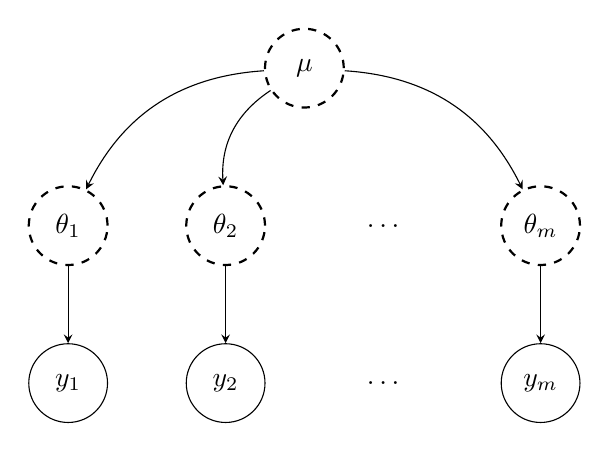
\begin{tikzpicture}[node distance=1cm,->,draw=black,>=stealth]
         % styles %
         \tikzstyle{param} = [circle,thick,draw=black,fill=white,dashed,minimum
         size=1cm];
         \tikzstyle{yobs} = [circle,draw=black,fill=white,minimum size=1cm];

         % nodes %
         \node [param] (mu) {$\mu$};

         \node [param,below of=mu, yshift=-1cm, xshift=-1cm] (theta2) {$\theta_2$};
         \node [param,draw=white,below of=mu, yshift=-1cm, xshift=1cm] (thetadots)
         {$\ldots$};
         \node [param,left of=theta2, xshift=-1cm] (theta1) {$\theta_1$};
         \node [param,right of=thetadots, xshift=1cm] (thetam) {$\theta_m$};

         \node [yobs,below of=theta1,yshift=-1cm] (y1) {$\vect y_1$};
         \node [yobs,below of=theta2,yshift=-1cm] (y2) {$\vect y_2$};
         \node [yobs,draw=white,below of=thetadots,yshift=-1cm] (ydots) {$\ldots$};
         \node [yobs,below of=thetam,yshift=-1cm] (ym) {$\vect y_m$};

         % edges %

         \path (mu)
         edge [bend right] node {} (theta1)
         edge [bend right] node {} (theta2)
         edge [bend left] node {} (thetam);
         \path (theta1) edge node {} (y1);
         \path (theta2) edge node {} (y2);
         \path (thetam) edge node {} (ym);
        \end{tikzpicture}
       \end{figure}
       Using this graph and its factorization one can calculate the conditioned
       probability as
       \begin{align*}
        p(\mu | \theta_1, \ldots, \theta_m, \tau^2, \sigma^2, \vect y_1, \ldots, \vect
        y_m)
         & = \frac{p(\mu, \theta_1, \ldots, \theta_m, \tau^2, \sigma^2, \vect y_1,
         \ldots,
         \vect y_m)}
        {p(\theta_1, \ldots, \theta_m, \tau^2, \sigma^2, \vect y_1, \ldots,
         \vect y_m)}
        \\
         & = \frac{p(\mu, \theta_1, \ldots, \theta_m, \tau^2, \sigma^2, \vect y_1,
         \ldots,
         \vect y_m)}
        {\int p(\mu, \theta_1, \ldots, \theta_m, \tau^2, \sigma^2, \vect y_1,
         \ldots, \vect y_m) \dd \mu}
        \\
         & = \frac{p(\vect y_1, \ldots, \vect y_m | \theta_1, \ldots, \theta_m, \sigma^2)
         \cdot
         p(\theta_1, \ldots, \theta_m | \mu, \tau^2) \cdot p(\mu)}
        {\int p(\vect y_1, \ldots, \vect y_m | \theta_1, \ldots, \theta_m,
         \sigma^2) \cdot
         p(\theta_1, \ldots, \theta_m | \mu, \tau^2) \cdot p(\mu) \dd \mu}
        \\
         & = \frac{p(\vect y_1, \ldots, \vect y_m | \theta_1, \ldots, \theta_m, \sigma^2)
         \cdot
         p(\theta_1, \ldots, \theta_m | \mu, \tau^2) \cdot p(\mu)}
        {p(\vect y_1, \ldots, \vect y_m | \theta_1, \ldots, \theta_m, \sigma^2)
         \cdot
         \int p(\theta_1, \ldots, \theta_m | \mu, \tau^2) \cdot p(\mu) \dd \mu}
        \\
         & = \frac{p(\theta_1, \ldots, \theta_m | \mu, \tau^2) \cdot p(\mu)}
        {\int p(\theta_1, \ldots, \theta_m | \mu, \tau^2) \cdot p(\mu) \dd \mu}
        \\
         & = \frac{p(\theta_1, \ldots, \theta_m, \mu, \tau^2)}{p(\theta_1, \ldots,
         \theta_m, \tau^2)}
        \\
         & = p(\mu | \theta_1, \ldots, \theta_m, \tau^2) \tag*{$ \square $}
       \end{align*}

       This result implies that the information obtained from the samples in a
       certain sense does not refer \textit{directly} on the grand mean, but it
       passes trough the inference that we do on $\theta$s. In fact, the grand mean
       is independent of the observations conditioned $ \theta_1, \ldots, \theta_m $.
\end{enumerate}

\section{Exercise on continuous mixture models}

\subsection{Data}
\begin{itemize}
 \item If $ y|\theta \sim \Poisson(\theta) $ and $ \theta \sim \Gammadist(\alpha,
       \beta) $, then the marginal (prior predictive) distribution of $ y $ is a
       negative binomial with parameters $\alpha$ and $\beta$ (or $ p = \beta / (1 +
       \beta) $).
 \item In the Normal model with unknown location and scale ($\mu$, $\sigma^2$),
       the non informative prior density, $ p(\mu, \sigma) \propto 1 / \sigma^2 $,
       results in a normal-inverse-$\chi^2$ posterior distribution. Marginally then
       $ \sqrt{n} (\mu - \bar y) / s $ has a posterior distribution $ t_{n - 1} $,
       where $ s^2 = \sum_i (y_i - \bar y)^2 / (n - 1) $ is the sample
       variance of the observation.
\end{itemize}

\subsection{Questions}
\begin{enumerate}[label=\alph*)]
 \item Derive the mean and the variance of the negative binomial.
 \item Derive the first two moments of the latter distribution, stating the
       appropriate condition on $n$ for existence of both of them.
\end{enumerate}

\subsection{Solutions}
\begin{enumerate}[label=\alph*)]
 \item We can leverage on the property of the expected value that, given two variables
       $ X $ and $ Y $
       \begin{equation}\label{week7:eq_condexpectation}
        \E_X[X] = \E_Y[\E_X[X | Y]]
       \end{equation}
       Thus,
       \begin{align*}
        \E_y[y] & = \E_\theta[\E_y[y | \theta]] \\
                & = \E_\theta[\theta]           \\
                & = \frac{\alpha}{\beta}
       \end{align*}

       For the variance, we can refer to \ref{week7:eq_totalvariance} and consider
       $ X = y $ and $ Y = \theta $
       \begin{align*}
        \Var[y] & = \E[\Var[y | \theta]] + \Var[\E[y | \theta]]   \\
                & = \E[\theta] + \Var[\theta]                     \\
                & = \frac{\alpha}{\beta} + \frac{\alpha}{\beta^2} \\
                & = \frac{(1 + \beta) \alpha}{\beta^2}
       \end{align*}

       \textbf{Formal alternative} \quad Using the following parameterization:
       \[ p(x | \theta, r) = \binom{x - 1}{r - 1} \theta ^{r} (1 - \theta) ^{x - r} \]
       with $ \theta = \beta / ( 1 + \beta) $ and $ r = \alpha $.

       \begin{align*}
        \E[x] & = \sum_{x \in \Theta} x \cdot p(x)
        \\
              & = \sum_{x = r}^{\infty} x \cdot \binom{x - 1}{r - 1} \cdot \theta ^r (1 -
        \theta) ^{x - r}
        \\
              & = \sum_{x = r}^{\infty} x \cdot \frac{(x - 1)!}{(r - 1)!(x - r)!} \cdot
        \theta ^r (1 - \theta) ^{x - r}
        \\
              & = r \cdot \sum_{x = r}^{\infty} \frac{x!}{r!(x - r)!} \cdot \theta ^r (1
        -
        \theta) ^{x - r}
        \intertext{\raggedleft Increment the lower index of the summation
         \\
         and decrement the index in the summand}
              & = \frac{r}{\theta} \cdot \sum_{x = r + 1}^{\infty} \binom{x - 1}{(r + 1)
         -
         1}
        \theta ^{r + 1} (1 - \theta) ^{x - (r + 1)}
        \intertext{\raggedleft The series is the sum of the PDF function of a $
          \text{NegBin}(\theta, r + 1) $
         \\
         all along its support, thus it is equal to 1}
              & = \frac{r}{\theta}
       \end{align*}

       To obtain the variance we recur to the equality
       \begin{equation}\label{week7:eq_variance}
        \Var[X] = \E[X^2] - \E[X]^2
       \end{equation}
       so, we obtain first of all $ \E[X^2] $.
       \begin{align*}
        \E[X^2]          & = \sum_{x = r}^{\infty} x^2 \cdot \binom{x - 1}{r - 1} \cdot
        \theta ^r
        (1 - \theta) ^{x - r}
        \\
                         & = \sum_{x = r}^{\infty} [x(x + 1) - x] \binom{x - 1}{r - 1}
        \cdot \theta
        ^r (1 - \theta) ^{x - r}
        \\
                         & = \sum_{x = r}^{\infty} [x(x + 1)] \binom{x - 1}{r - 1} \cdot
        \theta ^r
        (1 - \theta) ^{x - r} -
        \sum_{x = r}^{\infty} x \cdot \binom{x - 1}{r - 1} \cdot \theta ^r (1 -
        \theta) ^{x - r}
        \\
        \intertext{\raggedleft Following the same reasoning of the mean
         expression:
         \\
         multiply and divide for $ r $ and then $ r + 1 $}
                         & = \frac{r(r + 1)}{\theta ^2} \sum_{x = r + 2} \binom{x + 1}{r
         + 1} \theta
        ^{x + 2} (1 - \theta) ^{x - (r + 2)} -
        \frac{r}{\theta}
        \\
                         & = \frac{r(r + 1)}{\theta ^2} - \frac{r}{\theta}
        \\
                         & = \frac{r^2 + r - \theta r}{\theta ^2}
        \\
                         & = \frac{r^2}{\theta^2} + \frac{(1 - \theta) r}{\theta^2}
        \\
        \intertext{\raggedleft Now we can apply \ref{week7:eq_variance}}
        \implies \Var[X] & = \frac{r^2}{\theta^2} + \frac{(1 - \theta) r}{\theta^2} -
        \left( \frac{r}{\theta} \right)^2
        \\
                         & = \frac{(1 - \theta)r}{\theta ^ 2}
       \end{align*}
 \item The PDF of Student's t distribution
       \[ p(x | n) = c \cdot \left( 1 + \frac{x^2}{n} \right)^{-\frac{n + 1}{2}} \]
       where the c is a constant
       \[ c = \frac{1}{\sqrt{n}} \frac{1}{\Beta\left( \frac{n}{2}, \frac{1}{2}
       \right)} \]
       and $ \Beta(\parm, \parm) $ is the Beta function.

       It's immediate to see that the function is even, because $ x $ is present
       only as $ x^2 $, hence $ f(-x) = f(x) $.
       \begin{align*}
        \E[X] & = \int_{x \in \Theta} x \cdot f(x)  \dd x                         \\
              & = \int_{-\infty}^{\infty} x \cdot f(x) \dd x                      \\
              & = \int_{-\infty}^{0} x \cdot f(x) \dd x +
        \int_{0}^{\infty} x \cdot f(x) \dd x                                      \\
        \intertext{\raggedleft Change of variable in the first
         integral                                                                 \\$ t =
         -x $}
              & = -\int_{\infty}^{0} (-t) \cdot f(-t) \dd t +
        \int_{0}^{\infty} x \cdot f(x) \dd x                                      \\
              & = \phantom{-} \int_{\infty}^{0} \phantom{-} t \cdot f(-t) \dd t +
        \int_{0}^{\infty} x \cdot f(x) \dd x                                      \\
              & = -\int_{0}^{\infty} t \cdot f(-t) \dd t +
        \int_{0}^{\infty} x \cdot f(x) \dd x                                      \\
        \intertext{\raggedleft Since $ f(x) = f(-x) $}
              & = -\int_{0}^{\infty} t \cdot f(t) \dd t + \int_{0}^{\infty} x
        \cdot f(x) \dd x = 0
       \end{align*}
       The equality to 0 is granted by the finiteness of the two integrals, that
       is true only if the parameter $ n $ of the distribution is strictly
       greater then 1. In fact
       \begin{align*}
        \int_{0}^{\infty} x f(x) \dd x
         & = \lim\limits_{u \to \infty} \int_{0}^{u} x \cdot c \cdot
        \left( 1 + \frac{x^2}{n} \right)^{-\frac{1}{2}(n + 1)} \dd x    \\
         & = c \cdot \lim\limits_{u \to \infty} \left.
        -\frac{n}{n - 1} \left( 1 + \frac{x^2}{n} \right)^{-\frac{1}{2}(n - 1)}
        \right| _{0} ^{u}                                               \\
         & = -\frac{c \cdot n}{n - 1} \left( \lim\limits_{u \to \infty}
        \left( 1 + \frac{u^2}{n} \right)^{-\frac{1}{2}(n - 1)} - 1 \right)
       \end{align*}
       And the above limit is finite only if $ n > 1 $.

       \begin{align*}
        \E[X^2]
         & = \int_{x \in \Theta} x^2 \cdot f(x) \dd x
        \\
         & = \int_{-\infty}^{\infty} x^2 \cdot c \cdot \left( 1 + \frac{x^2}{n}
        \right)^{-\frac{n + 1}{2}} \dd x
        \intertext{\raggedleft Change of variable $ t = \left( 1 + \frac{x^2}{n}
          \right)^{-1} $}
         & = n ^{\frac{3}{2}} \cdot c \cdot \int_{0}^{1} t ^{\frac{n}{2} - 2} (1 - t)
        ^{\frac{1}{2}} \dd t
        \\
        \intertext{\raggedleft Note that the integrand function is the kernel of a Beta
         distribution,
         \\
         thus its result is known.}
         & = n ^{\frac{3}{2}} \cdot c \cdot \Beta\left( \frac{n}{2} - 1, \frac{3}{2}
        \right)
        \\
         & = n ^{\frac{3}{2}} \cdot \frac{1}{\sqrt{n} \Beta\left( \frac{n}{2},
         \frac{1}{2}
         \right)} \cdot
        \Beta\left( \frac{n}{2} - 1, \frac{3}{2} \right)
        \\
         & = n \cdot \frac{\Gamma\left( \frac{n}{2} + \frac{1}{2} \right)}
        {\Gamma\left( \frac{n}{2} \right) \Gamma\left( \frac{1}{2}
         \right)}
        \frac{\Gamma\left( \frac{n}{2} - 1 \right) \Gamma\left( \frac{3}{2}
         \right)}
        {\Gamma\left( \frac{n}{2} + \frac{1}{2} \right)}
        \\
        \intertext{\raggedleft By the property of the Gamma function that
         \\
         $ \Gamma(x) = (x - 1) \Gamma(x - 1) $}
         & = n \cdot \frac{\Gamma\left( \frac{n}{2} - 1 \right) \frac{1}{2} \Gamma\left(
         \frac{1}{2} \right)}
        {\left(\frac{n}{2} - 1\right) \Gamma\left( \frac{n}{2} - 1
         \right) \Gamma\left( \frac{1}{2} \right)}
        \\
         & = \frac{n}{n - 2}
       \end{align*}
       In this case the condition is $ n > 2 $, otherwise the integral of the
       Beta distribution does not converge.
\end{enumerate}
